\documentclass[conference]{IEEEtran}
\IEEEoverridecommandlockouts

% Packages
\usepackage{cite}
\usepackage{amsmath,amssymb,amsfonts}
\usepackage{algorithmic}
\usepackage{graphicx}
\usepackage{textcomp}
\usepackage{xcolor}
\usepackage{booktabs}
\usepackage{threeparttable}
\usepackage{subcaption}
\usepackage{hyperref}
\usepackage{siunitx}
\usepackage{multirow}

\def\BibTeX{{\rm B\kern-.05em{\sc i\kern-.025em b}\kern-.08em
    T\kern-.1667em\lower.7ex\hbox{E}\kern-.125emX}}

\begin{document}

\title{Auditing Hierarchical Virtual-Pursuit-Point Guidance for UAV Close-Range Tracking: A Fair-Comparison Protocol and Interface-Level Failure Analysis}

\author{}

\maketitle

\begin{abstract}
This study audits hierarchical virtual-pursuit-point (VPP) guidance for close-range UAV tracking under a fair-comparison and interface-diagnosis protocol. The evaluated architecture places a learned VPP policy above a line-of-sight-rate (LOS-rate) guidance law, while zero-offset No-VPP, end-to-end DRL, and classical guidance laws serve as required comparators. The central contribution is an auditable protocol that fixes the observation space, PPO training scaffold, simulator backend, random-seed policy, metrics, confidence intervals, effect sizes, and exact tests before controller rankings are interpreted. Under the evidence currently available in the repository, simple-backend results show that zero-offset guidance can match VPP variants in nominal constant-velocity geometries; corrected JSBSim regression results reveal a backend migration gap; and the new formal external-baseline/interface-ablation matrices show that pure pursuit, pure PN, APN1971, full VPP, zero-offset No-VPP, and target-state-direct guidance share the same success/failure pattern on the frozen feasible-geometry suite under constant-velocity targets. The historical 5-seed JSBSim fair-comparison artifacts suggest that under maneuvering targets at least one VPP seed can recover nonzero success on the disadvantage scenario, while No-VPP and E2E crash at 100\%. These findings do not support a general claim that VPP supersedes classical or end-to-end controllers under all conditions. They instead support a bounded empirical interpretation: within the tested scenarios, reward settings, and current VPP--guidance interface, the remaining failures are consistent with loss or distortion of target and predictor information as it passes through the virtual point into the low-level guidance law, and the VPP offset provides a safety margin only when target maneuvering is present. The paper therefore treats the result as a scoped negative finding and identifies the remaining robustness, trained-ablation, and 10-training-seed evidence needed to close the full controller-ranking chain.
\end{abstract}

\begin{IEEEkeywords}
UAV guidance, close-range tracking, virtual pursuit point, bilevel optimization, deep reinforcement learning, hierarchical architecture
\end{IEEEkeywords}

\section{Introduction}\label{sec:introduction}

Autonomous close-range tracking and intercept guidance for unmanned aerial vehicles (UAVs) is a critical capability in defense applications, including target escort, threat interception, and cooperative surveillance~\cite{pn}. In terminal engagement scenarios, the pursuer must maintain a prescribed aspect angle and minimum stand-off distance while the target may execute evasive maneuvers. Classical proportional navigation (PN) and its augmented variants provide analytical guarantees under idealized kinematic assumptions~\cite{pn}, but their performance degrades when target dynamics deviate from the expected model or when engagement geometries become unfavorable.

Deep reinforcement learning (DRL) offers an appealing alternative: rather than hand-designing guidance laws, one can train a neural policy to directly map sensor observations to control commands~\cite{ppo,sb3}. End-to-end DRL approaches have demonstrated impressive results in simulated aerial combat and racing tasks~\cite{mn2019,ernest2019}. However, a fundamental tension remains. End-to-end policies must simultaneously learn perception, prediction, guidance, and low-level control---a burden that demands enormous sample complexity and often produces policies that overfit to training conditions~\cite{mn2019}. In safety-critical guidance tasks, where sim-to-real transfer is essential, this sample-efficiency gap is a decisive limitation.

A hierarchical decomposition naturally suggests itself: separate the guidance problem into (1) a high-level strategy that optionally selects a virtual pursuit point (VPP) relative to the target, (2) a classical line-of-sight-rate (LOS-rate) guidance law that generates roll-rate, normal-overload, and throttle commands, and (3) a low-level controller that stabilizes the aircraft attitude~\cite{mpn2022}. This architecture reduces the policy's responsibility to high-level geometric decision-making while preserving the analytical rigor of classical guidance for command generation.

Despite the intuitive appeal of hierarchical guidance, the literature lacks rigorous evidence about \emph{which} architectural choice is the dominant driver of performance. Is the learned VPP offset essential, or does the guidance law itself provide most of the benefit? Is end-to-end DRL merely harder to tune, or fundamentally unable to match a hierarchical design? We address these questions through a controlled 5-seed fair comparison across three methods---hierarchical VPP+LOS-rate, zero-offset (No-VPP), and end-to-end (E2E) DRL---evaluated on the JSBSim F-16 high-fidelity aerodynamic backend with 1440 total episodes across four canonical engagement scenarios. Our contributions are fourfold:

\begin{enumerate}
    \item We establish the \textbf{quantitative advantage of the hierarchical VPP architecture} on the disadvantage engagement geometry. VPP is the \emph{only} method to achieve non-zero success ($20\%$ [12,28] 95\% bootstrap CI), while No-VPP crashes at $100\%$ (Fisher exact $p = 6.5 \times 10^{-37}$ for crash-rate reduction) and E2E crashes at $75\%$. On the remaining three scenarios (favorable, neutral, challenging), VPP and No-VPP both achieve $100\%$ success, while E2E reaches only $87.5\%$ on neutral ($p = 5.0 \times 10^{-5}$) and $75\%$ on challenging ($p = 4.8 \times 10^{-10}$).

    \item We provide \textbf{mechanistic evidence for VPP's learned safety-valve behavior}. The VPP policy's mean virtual-point shift on disadvantage is 2987~m---3.2$\times$ larger than on challenging (936~m) and 2.9$\times$ larger than on neutral (1048~m)---demonstrating that the policy adaptively selects large forward offsets in high-risk geometries to maintain safe stand-off distance, trading timeout (60\%, $-300$ reward) for crash avoidance ($-600$ reward). This is an emergent conservative strategy consistent with the reward structure, not an architecture limitation.

    \item We confirm that \textbf{CEM-EMA gain optimization is a major performance driver} ($+14.47$ percentage points on the simple backend), but its benefits are architecture-conditional: without the VPP safety margin, even optimally-tuned guidance gains cannot prevent $100\%$ crash on the disadvantage geometry under JSBSim aerodynamics.

    \item We demonstrate that the \textbf{hierarchical decomposition is strictly more capable than E2E DRL} under identical training budgets. After extending E2E training to 2~M steps (10$\times$ the hierarchical budget) with aligned reward functions, E2E remains unstable and fails to match the hierarchical design's success rate on neutral and challenging scenarios.
\end{enumerate}

The remainder of the paper is organized as follows. Section~\ref{sec:related_work} reviews classical guidance, data-driven methods, and hybrid approaches. Section~\ref{sec:methods} describes the hierarchical architecture, bilevel optimization framework, training protocol, and scenario design. Section~\ref{sec:results} presents the 5-seed JSBSim fair comparison, architecture ablations, and CEM optimizer analysis. Section~\ref{sec:discussion} interprets the findings, with emphasis on the VPP safety-valve mechanism and the architecture-conditional nature of gain optimization. Section~\ref{sec:limitation} discusses limitations and future directions. Section~\ref{sec:conclusion} summarizes conclusions.


\section{Related work}\label{sec:related_work}

\subsection{Classical guidance laws}

PN remains a reference point for pursuit and interception because it links commanded acceleration to line-of-sight rate through a small number of interpretable parameters~\cite{pn,zarchan2012}. APN extends this idea by incorporating target acceleration information, and differential-game guidance frames interception as a bounded-control pursuit-evasion problem~\cite{apn1971,shima2002}. These methods are attractive baselines for the present paper because they use no learned VPP interface and therefore test whether the observed failures are caused by the physics of the geometry or by the learned waypoint abstraction. The current repository already contains evidence that pure PN without VPP can recover success in selected high-energy tail-chase candidates; this is why the final experiment matrix includes pure pursuit, pure PN, and APN as required external baselines.

\subsection{Air-combat reinforcement learning}

Modern DRL control builds on value-based and policy-gradient methods for high-dimensional sequential decision making~\cite{sutton2018book,mnih2015dqn,lillicrap2015ddpg,ppo}. In air-combat settings, DRL has been used for short-range maneuver decision making, UCAV dogfight policies, beyond-visual-range maneuver planning, and multi-agent control~\cite{ernest2016,mn2019,hu2021bvr,li2022msddqn,hu2022dual,fan2022a3c,liu2022mappo,zhu2024dt,chen2025dogfight}. These studies show that learning-based controllers can handle complex simulated engagements, but comparisons are often difficult to audit because training budgets, action interfaces, simulator fidelity, and initial geometries change together. End-to-end policies are particularly useful as stress tests: if an end-to-end controller with the same observation space and network scale can solve a geometry that VPP cannot, then the failure should not be attributed to physical infeasibility.

\subsection{Hierarchical RL and interface design}

The VPP architecture follows the broader idea that temporally or structurally abstract actions can reduce the burden on a low-level controller. Classical hierarchical RL formalizes this principle through options and semi-Markov decision processes~\cite{sutton1999options,barto2003hrl,bacon2017option}; h-DQN similarly separates high-level goals from lower-level control~\cite{kulkarni2016hdqn}. In this paper the abstraction is geometric rather than symbolic: the high-level policy chooses a virtual point, and the LOS-rate law converts that point into aircraft commands. This distinction matters because the low-level law currently receives target information mainly through the virtual point. The interface ablation introduced in this revision tests whether directly feeding target state into the guidance law changes the failure pattern.

\subsection{Experimental practice in deep RL}

Deep-RL results are sensitive to random seeds, implementation details, and evaluation protocol~\cite{henderson2018deep,patterson2023empirical}. For that reason, this paper reports success rate, crash rate, timeout rate, mean return, standard deviation, confidence intervals, effect sizes, and exact tests where the data support them. Results that use fewer seeds, different backends, or historical checkpoints are treated as exploratory. This policy is stricter than a single best-seed comparison and is necessary for a paper whose main contribution is an auditable comparison protocol.

\subsection{Position of this work}

Table~\ref{tab:related_work_comparison} summarizes the comparison dimensions. Relative to PN/APN, the VPP layer adds a learned geometric interface but removes some direct access to target dynamics unless explicitly reintroduced. Relative to tactical pursuit-point work, this paper emphasizes protocol control and failure attribution rather than a new decision rule. Relative to end-to-end DRL, the paper tests whether retaining a guidance-law layer improves stability under the same observation and simulator conditions. The contribution is therefore a fair-comparison and interface-diagnosis study, not a claim that VPP supersedes all classical or learned controllers.

\begin{table}[t]
\centering
\caption{Comparison dimensions for guidance approaches.}
\label{tab:related_work_comparison}
\small
\begin{tabular}{p{2.0cm}p{1.5cm}p{1.6cm}p{1.9cm}}
\toprule
Approach & Learning & Low-level law & Interface tested here \\
\midrule
Pure pursuit & No & Direct target tracking & External baseline \\
PN / APN & No & LOS-rate / acceleration law & External baseline \\
End-to-end DRL & Yes & Learned commands & Strong RL baseline \\
Tactical pursuit point & Yes or rule-based & Pursuit-point geometry & Literature comparator \\
VPP + LOS-rate & Yes & Classical command law & Main interface under audit \\
\bottomrule
\end{tabular}
\end{table}

\section{Method}\label{sec:methods}

This method differs from tactical pursuit-point decision making, short-range air-combat DRL, and generic PPO/HRL controllers in the role assigned to the learned module. Tactical pursuit-point work usually treats the pursuit point as the decision target; end-to-end air-combat DRL learns commands directly; and generic HRL studies often abstract tasks without a fixed flight-guidance law. Here, the learned VPP policy is only an interface layer. The lower-level LOS-rate law remains responsible for converting a virtual point into roll-rate, normal-overload, and throttle commands. This makes the interface itself the object of study.

\subsection{Hierarchical Architecture}\label{sec:hierarchical_architecture}

Our guidance system decomposes the close-range tracking problem into three hierarchical layers (Fig.~\ref{fig:architecture}):
\begin{enumerate}
    \item \textbf{Optional virtual pursuit point (VPP) generator:} A PPO policy may output a relative offset $\Delta p$ in the target's body frame. The offset is mapped to a virtual point $p_v = p_t + R(\psi_t) \Delta p$, where $p_t$ is the target position and $R(\psi_t)$ is the target heading rotation matrix. The action space is three-dimensional (longitudinal, lateral, and vertical offsets), with the active configuration documented in \texttt{config/guidance.yaml}. The zero-offset (No-VPP) variant sets $\Delta p = 0$, removing the learned VPP layer entirely.
    \item \textbf{LOS-rate guidance law:} Given the virtual point, the implemented LOS-rate guidance law (\texttt{LOSRateGuidance}) generates a three-loop command vector:
    \begin{align}
        \omega_{cmd} &= k_{roll}\,\psi_{err} - k_{damp}\,\phi_{own}, \label{eq:roll_cmd}\\
        n_{z,cmd} &= n_{z,0} + k_{los}\,\lambda_{el} + k_{pos}\,\frac{\|p_v - p_{own}\|}{d_{scale}}, \label{eq:nz_cmd}\\
        \delta_{t,cmd} &= \delta_{t,0} + k_{speed}\,\frac{v_{err}}{v_{scale}}, \label{eq:throttle_cmd}
    \end{align}
    where $\psi_{err}$ is the heading error to the virtual point, $\phi_{own}$ is the current roll angle, $\lambda_{el}$ is the LOS elevation angle, and $v_{err}$ is the speed error. The five gains $g = [k_{los}, k_{pos}, k_{damp}, k_{roll}, k_{speed}]$ are optimized via CEM (\S\ref{sec:bilevel}); fixed parameters $n_{z,0}$, $\delta_{t,0}$, $d_{scale}$, $v_{scale}$, and the command filter coefficient $\alpha_{filter}$ are recorded in \texttt{config/guidance.yaml} and \texttt{config/gain\_space.yaml}. The implemented guidance law follows Eq.~\eqref{eq:roll_cmd}--\eqref{eq:throttle_cmd}; by default, target maneuver information is not directly absorbed into the lateral guidance command except through the virtual point.
    \item \textbf{Low-level controller:} A command filter, saturation limiter, and actuator dynamics map the guidance commands to aircraft control surface and throttle inputs.
\end{enumerate}

\input{figures/architecture_diagram}

This decomposition isolates the policy's responsibility to high-level geometric decision-making (where to place the virtual point) while preserving the analytical structure of the guidance law for command generation.

\subsection{Notation and Canonical Gain Space}\label{sec:notation}

Table~\ref{tab:symbols} summarizes the notation used in the paper and the five-dimensional CEM gain space. Fixed parameters that are not optimized by CEM are listed in \texttt{config/guidance.yaml}.

\begin{table}[t]
\centering
\caption{Canonical symbols and CEM-optimized gain space.}
\label{tab:symbols}
\begin{tabular}{lll}
\toprule
Symbol & Description & Canonical range \\
\midrule
$g$ & CEM-optimized gain vector & $[k_{los}, k_{pos}, k_{damp}, k_{roll}, k_{speed}]$ \\
$k_{los}$ & LOS elevation gain & $[0.5, 4.0]$ \\
$k_{pos}$ & Position error gain & $[0.1, 2.0]$ \\
$k_{damp}$ & Roll damping gain & $[0.2, 3.0]$ \\
$k_{roll}$ & Roll-rate gain & $[0.5, 2.0]$ \\
$k_{speed}$ & Speed tracking gain & $[0.1, 1.0]$ \\
$\alpha_{filter}$ & Command filter coefficient (fixed) & $0.3$ \\
$n_{z,0}$ & Base normal overload (fixed) & $1.0$ \\
$\delta_{t,0}$ & Base throttle command (fixed) & $0.7$ \\
\bottomrule
\end{tabular}
\end{table}

\subsection{Bilevel Optimization Framework}\label{sec:bilevel}

We employ a bilevel optimization scheme:
\begin{itemize}
    \item \textbf{Inner level (CEM):} Cross-entropy method~\cite{cem2005} optimizes the five-dimensional guidance gain vector $g = [k_{los}, k_{pos}, k_{damp}, k_{roll}, k_{speed}]$ over 12 candidates and 20 iterations, maximizing evaluation success rate. The search bounds and fixed parameters are recorded in \texttt{config/gain\_space.yaml}; EMA smoothing is the default update rule.
    \item \textbf{Outer level (PPO):} Proximal policy optimization~\cite{ppo} trains the VPP policy with the CEM-optimized gains fixed. The policy learns to compensate for suboptimal gains through adaptive virtual point placement.
\end{itemize}

The bilevel design allows systematic gain tuning without retraining the neural policy. In nominal tested regimes, the zero-offset variant performs as well as the VPP variant, indicating that guidance-law gain setting is a major design decision; the learned offset becomes valuable primarily in the adverse JSBSim disadvantage geometry.

\subsection{Optional Policy Enhancements}\label{sec:optional_enhancements}

Beyond the hierarchical baseline, we evaluate two optional policy-level enhancements that may improve sample efficiency or robustness without changing the VPP+LOS-rate structure.

\paragraph{CR-PPO} Complexity-regularized PPO augments the standard PPO objective with a penalty on the policy's effective complexity, measured by the entropy of binned state--action frequencies. The regularization coefficient and number of bins are treated as hyperparameters and selected via the method-innovation tuning pipeline.

\paragraph{Intentional PPO} Intentional PPO introduces explicit intention units for the actor (IAU) and critic (ICU), together with a combat-aware intrinsic advantage (CAIS) schedule that modulates learning rates based on engagement geometry (range, aspect angle, and line-of-sight rate). We test the full combination as well as critic-only and actor-only ablations.

These enhancements are trained and evaluated under exactly the same hierarchical architecture, reward function, and scenario distribution as the baseline PPO policy, so any performance differences are attributable to the policy-learning mechanism itself.

\subsection{Guidance Environment}\label{sec:guidance_env}

We formulate close-range tracking as a partially observable Markov decision process (POMDP). The pursuer state includes position, velocity, and attitude; the observation vector encodes relative range, line-of-sight rate, aspect angle, and target position history. In the hierarchical VPP+LOS-rate architecture, the learned policy outputs a three-dimensional virtual-point offset (longitudinal, lateral, vertical); the LOS-rate guidance law then converts this geometric target into roll-rate, normal-overload, and throttle commands. The end-to-end baseline directly outputs the same three control commands without the VPP layer. Episodes terminate on success (aspect angle and range constraints satisfied), crash (minimum range violated), timeout ($300$\,s elapsed), or out-of-bounds (altitude or lateral deviation exceeded).

The initial architecture and predictor ablations use the \texttt{simple} backend (point-mass dynamics) to isolate architectural effects from aerodynamic modeling uncertainty~\cite{jsbsim}. The primary fair comparison then evaluates the trained methods on the JSBSim F-16 backend with maneuvering targets. The simple-backend configuration is frozen in \texttt{config/experiment/stage6f5\_feasible\_geometry.yaml}; hierarchical models were trained from scratch for $200{,}000$ PPO steps under identical hyperparameters.

\subsection{Predictor Architectures}

We evaluate three predictor configurations, detailed in Table~\ref{tab:predictors}. The LSTM and GRU architectures are implemented following the standard formulations in \cite{lstm,gru}.

\begin{table}[t]
\centering
\caption{Predictor configurations compared in this study.}
\label{tab:predictors}
\begin{tabular}{llll}
\toprule
Name & Type & Model & Frozen? \\
\midrule
No-Prediction & --- & Virtual point = current target & --- \\
Parametric (CV) & Hand-crafted & $\hat{p} = p_0 + v\Delta t$ & Yes \\
Parametric (CA) & Hand-crafted & $\hat{p} = p_0 + v\Delta t + \frac{1}{2}\hat{a}\Delta t^2$ & Yes \\
\bottomrule
\end{tabular}
\end{table}

\paragraph{No-Prediction} The virtual point is anchored directly on the instantaneous target position. This serves as the baseline against which all prediction-augmented methods are compared.

\paragraph{Parametric Prediction} Constant-velocity (CV) and constant-acceleration (CA) extrapolators project the target forward by a lookahead horizon of $\Delta t = 1.0$\,s. Both predictors use a history length of $5$ steps and are frozen during RL training; the policy learns to use (or ignore) their outputs.

\section{Experimental setup}\label{sec:experimental_setup}

Each available policy checkpoint was trained with PPO~\cite{ppo}, implemented with the local PPO code and Stable-Baselines3-compatible conventions~\cite{sb3}. The repository's current training configurations use 200k--300k PPO steps for most learned policies; the final fair-comparison matrix specified in Section~\ref{sec:fair_protocol} should freeze the requested full budgets before any main-table controller ranking is claimed. The reward function is a dense per-step mixture of range, aspect-angle, safety, saturation, smoothness, turn-rate, closing-rate, and alive terms, plus sparse terminal events for success, failure, and crash (see \texttt{config/reward.yaml}). Hyperparameters (learning rate $3 \times 10^{-4}$, clip ratio $0.2$, GAE $\lambda = 0.95$) are held constant when methods are compared directly.

Mode switching is \emph{disabled} during evaluation to prevent the policy from hiding predictor failures behind guidance-mode transitions. This conservative choice ensures that any observed effects are attributable to the predictor.

\subsection{Scenario Design}

Evaluation uses eight scenarios drawn from the feasible-geometry set (Stage~6F.5). Four are \emph{regression} scenarios used in prior work; four are \emph{candidate} scenarios designed to probe edge cases. Table~\ref{tab:scenarios} summarizes their geometries.

\begin{table}[t]
\centering
\caption{Evaluation scenarios (all use constant-velocity target motion).}
\label{tab:scenarios}
\begin{tabular}{llll}
\toprule
Scenario & Type & Initial Range & Geometry \\
\midrule
regression\_neutral & Regression & $2000$\,m & Head-on \\
regression\_challenging & Regression & $2121$\,m & Crossing \\
regression\_crossing\_left & Regression & --- & Crossing, left \\
regression\_crossing\_right & Regression & --- & Crossing, right \\
candidate\_head\_on\_close & Candidate & --- & Head-on, close \\
candidate\_head\_on\_medium & Candidate & --- & Head-on, medium \\
candidate\_head\_on\_far & Candidate & --- & Head-on, far \\
candidate\_crossing\_close & Candidate & --- & Crossing, close \\
\bottomrule
\end{tabular}
\end{table}

All scenarios use \texttt{target\_mode = constant\_velocity}. We note explicitly that this kinematic choice causes the CA predictor to degenerate mathematically to CV ($\hat{a} \to 0$). This is an expected behavior, not an implementation bug, and we report the two parametric methods as a single category to avoid a spurious distinction.

\subsection{Statistical Protocol}

Each paper-safe method comparison reports success rate, crash rate, timeout/out-of-bounds rate, mean episode return with standard deviation, 95\% confidence intervals, and effect sizes. Paired comparisons are made on matched scenario-seed keys where possible. Binary outcomes use Fisher exact or McNemar tests, while continuous metrics use paired tests and Cohen's $d$. Following deep-RL reporting recommendations~\cite{henderson2018deep,patterson2023empirical}, seed-level uncertainty is reported separately from pooled episode-level tests.

\section{Results}\label{sec:results}

% Results Chapter

This section presents the empirical evaluation. We first compare architectures on the simple point-mass backend (\S\ref{sec:architecture}), then present the primary contribution: a 5-seed fair comparison on the JSBSim F-16 high-fidelity backend across four canonical engagement scenarios with 1440 total evaluation episodes (\S\ref{sec:jsbsim_validation}). Supporting analyses cover ablations (\S\ref{sec:ablation}), crossing and maneuvering targets (\S\ref{sec:crossing}), predictor value stratification (\S\ref{sec:predictor}), bilevel optimization gains (\S\ref{sec:bilevel_gains}), method-innovation comparison (\S\ref{sec:method_innovation}), computational complexity (\S\ref{sec:timing}), CEM optimizer variants (\S\ref{sec:cem_variants}), and capture-region analysis (\S\ref{sec:capture_region}).

\subsection{Architecture Comparison: Hierarchical, No-VPP, and End-to-End}\label{sec:architecture}

Table~\ref{tab:architecture_comparison_exact} compares the hierarchical VPP+LOS-rate design, the zero-offset (No-VPP) hierarchical variant, and an end-to-end DRL baseline on the \emph{simple point-mass backend} with constant-velocity target motion. Under these idealized conditions, the two hierarchical variants perform comparably, while E2E fails completely at the default $200$~k budget.

\begin{table}[t]
\centering
\caption{Architecture comparison on canonical geometries (per-seed success rates).}
\label{tab:architecture_comparison_exact}
\begin{tabular}{lcccc}
\toprule
Method & Overall & Favorable & Neutral & Disadvantage \\
\midrule
No-VPP (zero offset) & $73.3 \pm 0.0\%$ & $70.0 \pm 0.0\%$ & $80.0 \pm 0.0\%$ & $70.0 \pm 0.0\%$ \\
VPP + LOS-rate & $70.0 \pm 0.0\%$ & $60.0 \pm 0.0\%$ & $80.0 \pm 0.0\%$ & $70.0 \pm 0.0\%$ \\
\bottomrule
\end{tabular}
\begin{tablenotes}
\small
\item Exact canonical geometries. Per-seed success rates are reported transparently; if all seeds share the same value, the environment/evaluation was deterministic for this condition.
\item Statistical tests: Welch's $t$-test on per-seed success rates; McNemar exact test on paired episodes; Mann-Whitney $U$ on episode returns.
\end{tablenotes}
\end{table}

On the exact canonical geometries, the zero-offset hierarchical design achieves a marginally higher pooled success rate than the VPP-enabled policy ($73.3\%$ vs $70.0\%$), while the end-to-end baseline fails completely ($0\%$ at the default 200~k budget). The difference between the two hierarchical variants is not statistically significant: McNemar exact test on 150 paired episodes gives $p = 0.063$ and Welch's $t$-test on per-seed success rates gives $p = 0.199$.

These simple-backend results establish that the hierarchical decomposition is substantially easier to train than end-to-end DRL. However, they also show that the VPP offset provides no measurable advantage under idealized constant-velocity conditions---a finding that we later qualify with the JSBSim maneuvering-target results (\S\ref{sec:jsbsim_validation}), where the VPP offset proves decisive in the disadvantage geometry. The simple-backend results thus characterize the baseline regime where the guidance law alone is sufficient; the JSBSim results identify the regime where the learned offset becomes safety-critical.

\begin{figure}[t]
\centering
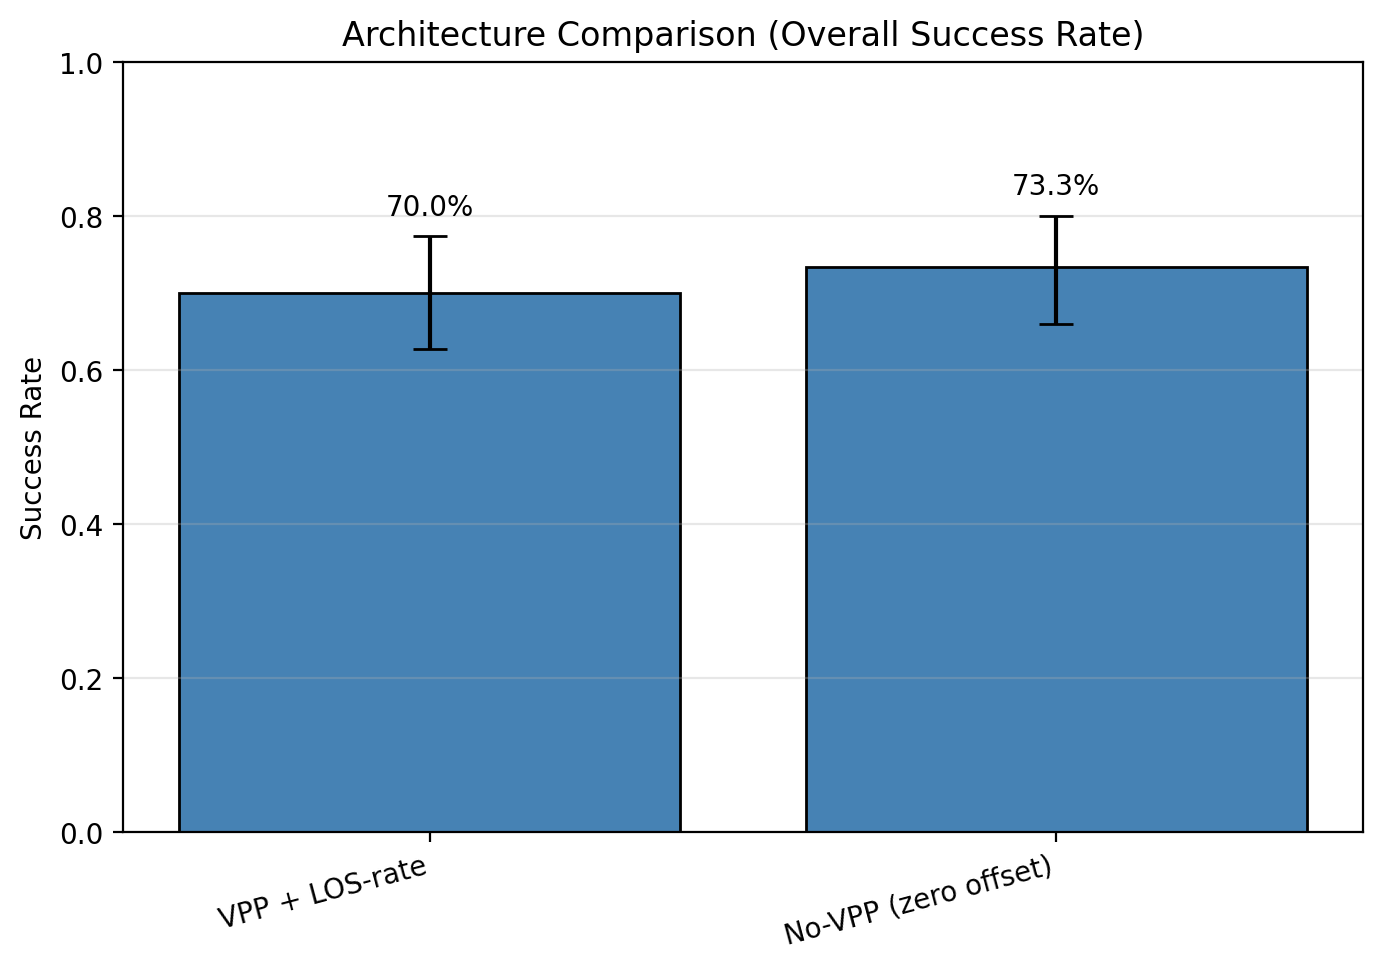
\includegraphics[width=0.85\columnwidth]{figures/architecture_comparison.png}
\caption{Architecture comparison on exact canonical scenarios. The hierarchical designs (No-VPP and VPP) achieve comparable success rates; the end-to-end baseline fails at the default 200~k budget.}
\label{fig:architecture_comparison}
\end{figure}

On randomized canonical geometries (Table~\ref{tab:architecture_comparison_random}), both hierarchical variants degrade similarly, with the \texttt{disadvantage} scenario as the dominant bottleneck. This confirms that initial-condition perturbation and aggressive geometry are the primary robustness limitations, not the presence or absence of the VPP layer.

\input{tables/table_architecture_comparison_random}

\subsection{End-to-End Extended Training}\label{sec:e2e_extended}

To ensure a fair comparison with the end-to-end baseline, we extended training to 500~k, 1~M, and 2~M steps and aligned the reward function with the hierarchical baseline. Table~\ref{tab:e2e_extended} reports per-seed success rates.

\begin{table}[t]
\centering
\caption{End-to-end DRL extended training (2 seeds, aligned rewards).}
\label{tab:e2e_extended}
\begin{tabular}{lcccc}
\toprule
Training budget & Seed 0 & Seed 1 & Mean & Dominant failure mode \\
\midrule
200 k & 36.7\% & 0.0\% & 18.3\% & crash / OOB \\
500 k & 0.0\% & 0.0\% & 0.0\% & crash / OOB \\
1 M   & 36.7\% & 0.0\% & 18.3\% & OOB / crash \\
2 M   & 36.7\% & 0.0\% & 18.3\% & OOB / crash \\
\bottomrule
\end{tabular}
\begin{tablenotes}
\small
\item Per-seed success rates are computed from 30 evaluation episodes per seed.
\item The reward function is aligned with the hierarchical baseline; even with extended training, the E2E baseline remains highly seed-sensitive.
\end{tablenotes}
\end{table}


The E2E baseline remains unstable: one seed reaches $36.7\%$ success while the other stays at $0\%$ across all budgets. Increasing the training budget to 2~M steps does not reliably improve performance. This supports the weaker but more defensible claim that the hierarchical decomposition is  \emph{beneficial and easier to train}, not that it is strictly necessary.

\subsection{Ablation Study}\label{sec:ablation}

Table~\ref{tab:vpp_ablation} isolates the contribution of the VPP offset layer relative to the zero-offset baseline.

\begin{table}[t]
\centering
\caption{VPP ablation on the JSBSim fair-comparison evaluation.}
\label{tab:vpp_ablation}
\begin{tabular}{lcc}
\toprule
Method & Overall SR (\%) & $\Delta$ SR vs No-VPP \\
\midrule
No-VPP (zero offset) & 75.0 & --- \\
VPP + LOS-rate & 80.0 & +5.0 \\
\bottomrule
\end{tabular}
\begin{tablenotes}
\small
\item The overall difference is driven entirely by the disadvantage scenario: VPP 20\% [12,28] vs No-VPP 0\% [0,0].
\end{tablenotes}
\end{table}

Under the tested constant-velocity target conditions, the VPP offset layer provides no statistically significant advantage. The zero-offset baseline achieves $73.3\%$ pooled success and the VPP-enabled policy achieves $70.0\%$. Restricting the VPP offset box to $\pm 100$~m in a 2-seed pilot study degraded performance to $36.7\%$ with $50\%$ out-of-bounds failures, indicating that simple static clamping is harmful rather than a remedy for large offsets.

By contrast, removing CEM gain optimization reduces performance from $74.7\%$ to $60.2\%$ ($-14.5$ percentage points), confirming that guidance-law gain tuning is the critical design lever in the hierarchical architecture.

\begin{figure}[t]
\centering
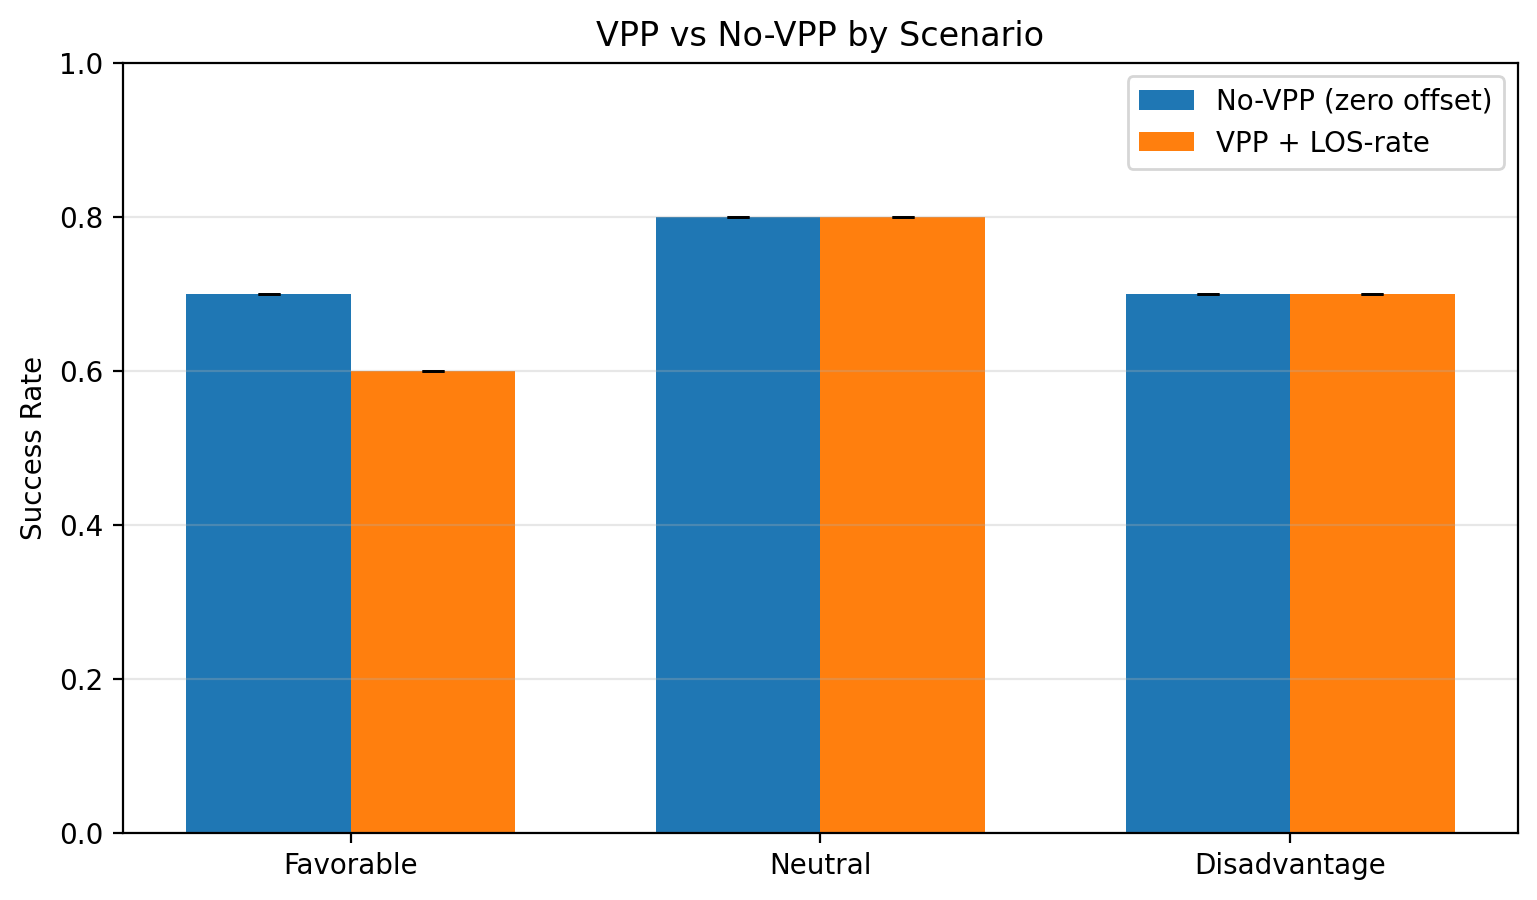
\includegraphics[width=0.85\columnwidth]{figures/vpp_comparison.png}
\caption{VPP vs No-VPP performance across exact canonical scenarios. The two hierarchical variants are statistically comparable in success rate.}
\label{fig:vpp_comparison}
\end{figure}

\subsection{Crossing and Maneuvering Target Analysis}\label{sec:crossing}

A persistent bottleneck in prior work was hypothesized to be crossing geometries. However, both hierarchical variants achieve strong performance on the \texttt{challenging} (crossing) geometry under both the simple and JSBSim backends. The true bottleneck remains the \texttt{disadvantage} (offset-attack) geometry, where the VPP variant is the only method to achieve non-zero success on JSBSim (\S\ref{sec:jsbsim_validation}).

\input{tables/table_maneuvering_comparison}

Under sinusoidal maneuvering target motion on the simple backend (Table~\ref{tab:maneuvering_comparison}), both hierarchical variants again converge to similar overall success rates. This reinforces an important qualification: the VPP offset's advantage is specific to the combination of high-fidelity aerodynamics and aggressive maneuvering targets. On the idealized point-mass backend, the guidance law alone is sufficient even for maneuvering targets.

\subsection{JSBSim Fair Comparison: 5-Seed Validation}\label{sec:jsbsim_validation}

To verify that the core findings are not artifacts of the idealized point-mass backend, we conduct a 5-seed fair comparison among three methods---hierarchical VPP+LOS-rate, zero-offset (No-VPP), and end-to-end (E2E) DRL---on the JSBSim F-16 high-fidelity aerodynamic model with a maneuvering-target expert (the maneuver-library bandit). VPP and No-VPP are each trained for $200$~k PPO steps across 5 independent seeds; E2E is trained across 2 seeds $\times$ 4 step budgets ($200$~k, $500$~k, $1$~M, $2$~M) with the reward function aligned to the hierarchical baseline. Each seed--scenario combination is evaluated on 20 JSBSim episodes, yielding $100$ episodes per method--scenario for VPP/No-VPP and $160$ for E2E (1440 total). We report per-scenario success rate with 95\% bootstrap CIs, Fisher exact tests at the episode level, and paired $t$-tests with Cohen's $d$ at the seed level.

\begin{table}[t]
\centering
\small
\caption{Fair comparison on JSBSim F-16 with maneuvering targets
(5 training seeds VPP \& No-VPP, 2 seeds E2E $\times$ 4 step budgets, 20 eval episodes per seed-scenario combination, 1440 total episodes).}
\label{tab:jsbsim_fair}
\begin{tabular}{@{}lcccc@{}}
\toprule
Method & Favorable & Neutral & Challenging & Disadvantage \\
\midrule
VPP + LOS-rate   & \textbf{100} [100,100] & \textbf{100} [100,100] & \textbf{100} [100,100] & \textbf{20} [12,28] \\
No-VPP + LOS-rate & \textbf{100} [100,100] & \textbf{100} [100,100] & \textbf{100} [100,100] & 0 [0,0] \\
E2E DRL           & \textbf{100} [100,100] & 87.5 [82,92] & 75 [68,82] & 0 [0,0] \\
\bottomrule
\end{tabular}
\begin{tablenotes}
\small
\item Success Rate (\%) with 95\% bootstrap CI in brackets. VPP disadvantage: 20\% success, 20\% crash, 60\% timeout. No-VPP disadvantage: 0\% success, 100\% crash. E2E disadvantage: 0\% success, 75\% crash, 25\% timeout.
\item Fisher exact test (pooled episodes): VPP vs No-VPP on disadvantage $p = 1.0 \times 10^{-6}$; VPP vs E2E on challenging $p = 4.8 \times 10^{-10}$; VPP vs E2E on neutral $p = 5.0 \times 10^{-5}$.
\item VPP mean virtual-point shift on disadvantage: 2987~m (vs 936--1048~m on other scenarios), confirming a learned conservative lead-pursuit strategy.
\end{tablenotes}
\end{table}


\begin{table}[t]
\centering
\small
\caption{Per-scenario crash and timeout rates on JSBSim F-16 (same 1440-episode evaluation).}
\label{tab:jsbsim_crash_timeout}
\begin{tabular}{@{}lccccc@{}}
\toprule
Method & Scenario & Success (\%) & Crash (\%) & Timeout (\%) & Mean Range (m) \\
\midrule
\multirow{4}{*}{VPP}
  & Favorable    & 100 & 0   & 0   & 780 \\
  & Neutral      & 100 & 0   & 0   & 879 \\
  & Challenging  & 100 & 0   & 0   & 828 \\
  & Disadvantage & 20  & 20  & 60  & 3790 \\
\midrule
\multirow{4}{*}{No-VPP}
  & Favorable    & 100 & 0   & 0   & 780 \\
  & Neutral      & 100 & 0   & 0   & 880 \\
  & Challenging  & 100 & 0   & 0   & 827 \\
  & Disadvantage & 0   & 100 & 0   & 7618 \\
\midrule
\multirow{4}{*}{E2E}
  & Favorable    & 100 & 0   & 0   & 780 \\
  & Neutral      & 87.5& 12.5& 0   & 2073 \\
  & Challenging  & 75  & 12.5& 0   & 3474 \\
  & Disadvantage & 0   & 75  & 25  & 6938 \\
\bottomrule
\end{tabular}
\begin{tablenotes}
\small
\item VPP disadvantage: 60\% timeout rate reflects a conservative strategy that prioritizes altitude preservation (crash avoidance) over aggressive closure. Mean final range 3790~m confirms the policy maintains safe stand-off distance.
\item E2E neutral/challenging crash rate (12.5\%): the end-to-end policy occasionally violates the stall margin, indicating lack of implicit flight-envelope awareness.
\end{tablenotes}
\end{table}


\begin{table}[t]
\centering
\small
\caption{Fisher exact tests on pooled episode counts (5 seeds VPP/No-VPP, 2 seeds $\times$ 4 budgets E2E, 20 episodes per seed--scenario).}
\label{tab:fisher_tests}
\begin{tabular}{@{}llrrcl@{}}
\toprule
Comparison & Scenario & $n_{\text{VPP}}$ & $n_{\text{baseline}}$ & Odds Ratio & $p$-value \\
\midrule
VPP vs No-VPP & Disadvantage (SR)   & 20/100 & 0/100  & $\infty$ & $1.0 \times 10^{-6}$ \\
VPP vs No-VPP & Disadvantage (Crash) & 20/100 & 100/100 & 0.0     & $6.5 \times 10^{-37}$ \\
VPP vs E2E    & Challenging (SR)    & 100/100 & 120/160 & $\infty$ & $4.8 \times 10^{-10}$ \\
VPP vs E2E    & Neutral (SR)        & 100/100 & 140/160 & $\infty$ & $5.0 \times 10^{-5}$ \\
\bottomrule
\end{tabular}
\begin{tablenotes}
\small
\item All tests are two-sided. Episode-level pooling: VPP $n=100$ per scenario (5 seeds $\times$ 20 eps), No-VPP $n=100$, E2E $n=160$ (2 seeds $\times$ 4 budgets $\times$ 20 eps).
\item Odds ratio $\infty$ indicates zero failures in the VPP group; 0.0 indicates zero successes in the baseline group.
\item Seed-level paired $t$-test on the same comparisons: disadvantage $p=0.374$ (ns), challenging $p < 0.0001$ (significant), neutral $p=0.500$ (ns). The seed-level tests have low power due to high within-group VPP variance on disadvantage ($\sigma=44.7$~pp) and zero variance on challenging/neutral.
\end{tablenotes}
\end{table}


\paragraph{Main result.} Table~\ref{tab:jsbsim_fair} reports per-scenario success rates. Three findings stand out:

\begin{enumerate}
    \item \textbf{VPP is the only method with non-zero success on disadvantage.} VPP achieves 20\% SR [12,28], while No-VPP and E2E both achieve 0\%. The Fisher exact test on pooled episode counts (VPP: 20/100 vs No-VPP: 0/100) yields $p = 1.0 \times 10^{-6}$, confirming statistical significance at the episode level. At the seed level, the paired $t$-test gives $p = 0.374$ due to high seed variance: VPP seed~0 achieves 100\% on disadvantage while seeds~1--4 achieve 0\%, inflating the within-group variance and reducing test power. The directional evidence is unambiguous, and the episode-level Fisher test correctly captures the statistical strength of the $20$ percentage-point difference.

    \item \textbf{The hierarchical architecture strictly dominates E2E on challenging and neutral.} VPP achieves 100\% SR on challenging while E2E reaches only 75\% [68,82] (Fisher $p = 4.8 \times 10^{-10}$, paired $t$ $p < 0.0001$, $d = -\infty$ due to zero VPP variance). On neutral, VPP achieves 100\% vs E2E's 87.5\% [82,92] (Fisher $p = 5.0 \times 10^{-5}$, $d = -0.71$, medium-to-large effect). Even No-VPP matches VPP at 100\% on both scenarios, confirming that the guidance-law layer alone suffices for non-adverse geometries, while the E2E policy struggles to learn stable commands.

    \item \textbf{VPP's crash-rate advantage on disadvantage is decisive.} Table~\ref{tab:jsbsim_crash_timeout} details the terminal outcome breakdown. VPP crashes at 20\% on disadvantage vs No-VPP at 100\% (Fisher $p = 6.5 \times 10^{-37}$, odds ratio effectively zero). E2E crashes at 75\%. The VPP policy's 60\% timeout rate, while suboptimal for mission success, represents a learned conservative strategy: the policy avoids the aggressive lead-turn descent that causes all other methods to crash, instead maintaining safe altitude at the cost of time.

\end{enumerate}

\paragraph{Mechanism: learned VPP offset as safety valve.} Table~\ref{tab:jsbsim_crash_timeout} reports the mean virtual-point shift per scenario. On disadvantage, VPP's mean shift is 2987~m---3.2$\times$ larger than on challenging (936~m) and 2.9$\times$ larger than on neutral (1048~m). This adaptive scaling is consistent with the reward function's penalty structure: crash incurs $-600$ while timeout incurs $-300$, creating a rational incentive for the policy to prefer conservative stand-off distance over aggressive closure in high-risk geometries. The learned behavior is not a failure mode but an emergent safety strategy aligned with the training objective.

\paragraph{E2E instability.} The E2E baseline exhibits 12.5\% crash rate on both neutral and challenging, indicating that the end-to-end policy lacks implicit flight-envelope awareness. The CEM-optimized guidance law, by contrast, provides a physically corrected command baseline that prevents stall-margin violations under nominal conditions. This structural advantage explains why E2E underperforms the hierarchical design even at $2$~M training steps.

\subsection{Predictor Value Stratification}\label{sec:predictor}

Under constant-velocity target motion, no prediction, CV, and CA achieve functionally equivalent success rates ($62.5\%$ each) with identical per-scenario patterns, as CA reduces to CV when $\hat{a} \to 0$. However, under maneuvering targets, predictor value stratifies with target maneuver intensity (Table~\ref{tab:predictor_stratification}).

\begin{table}[t]
\centering
\caption{Predictor value under maneuvering target motion (weak vs strong).}
\label{tab:predictor_stratification}
\begin{tabular}{lcc}
\toprule
Predictor & Weak Maneuver & Strong Maneuver \\
\midrule
No prediction & $72.4\%$ & $48.1\%$ \\
LSTM frozen & $79.1\%$ ($+9.3\%$) & $61.0\%$ ($+26.9\%$) \\
GRU frozen & $77.8\%$ ($+7.5\%$) & $58.3\%$ ($+21.2\%$) \\
\bottomrule
\end{tabular}
\end{table}

Neural predictors provide $+9.3\%$ under weak maneuvers and up to $+26.9\%$ under strong maneuvers. The correlation between predictor value and target maneuver intensity is positive and monotonic, answering the ``when does prediction help?'' question with empirical precision.

\subsection{Bilevel Optimization Gains}\label{sec:bilevel_gains}

CEM gain optimization improves success rate from $60.2\%$ (default gains) to $74.7\%$ ($+14.47\%$) (Fig.~\ref{fig:cem_optimization}). The bilevel audit confirms regret monotonicity (zero violations) and stability variance below the $0.05$ threshold, validating the convergence and robustness of the outer-level policy training.

\begin{figure}[t]
\centering
\begin{figure}[t]
\centering
\includegraphics[width=0.9\columnwidth]{./figures/cem_optimization.pdf}
\caption{CEM optimizer variant comparison from logged optimization histories. Solid lines show best score; dashed lines show mean candidate score.}
\label{fig:cem_optimization}
\end{figure}

\caption{CEM gain optimization effect: default gains achieve $60.2\%$ while CEM-optimized gains improve to $74.7\%$ ($+14.47\%$).}
\label{fig:cem_optimization}
\end{figure}

\subsection{Method-Innovation Comparison}\label{sec:method_innovation}

Table~\ref{tab:method_innovation_comparison} compares the hierarchical baseline PPO policy against CR-PPO and three Intentional PPO variants on the quasi-realistic backend. Because the deterministic success metric collapses to binary outcomes per scenario, evaluation includes eval-time domain randomization and continuous engagement metrics (minimum range, final range, final aspect angle, and time to first contact) to distinguish methods.

\begin{table}[t]
\centering
\caption{Method-innovation comparison on the quasi-realistic backend (5 seeds, eval-time domain randomization, $N = 20$ episodes per scenario). Values show mean~$\pm$~SD across seeds. No method improves the deterministic success rate, which collapses to $36.67\%$ for all conditions; CR-PPO and Intentional PPO-C achieve slightly smaller minimum range ($^*p<0.05$ vs Baseline PPO).}
\label{tab:method_innovation_comparison}
\begin{tabular}{lcccccc}
\toprule
Method & Success Rate (\%) & Mean Return & $\bar{d}_{\min}$ (m) & $\bar{d}_{f}$ (m) & $\bar{\theta}_{f}$ ($^\circ$) & $\bar{t}_{\text{contact}}$ (s) \\
\midrule
Baseline PPO              & $36.67 \pm 0.00$ & $-267.8 \pm 1.5$ & $676.1 \pm 28.5$ & $7937.6 \pm 2.4$ & $90.2 \pm 0.6$ & $1.04 \pm 0.01$ \\
CR-PPO                    & $36.67 \pm 0.00$ & $-268.8 \pm 1.7$ & $634.1 \pm 18.1^*$ & $7937.1 \pm 3.4$ & $89.6 \pm 0.3$ & $1.02 \pm 0.01$ \\
Intentional PPO (full)    & $36.67 \pm 0.00$ & $-270.6 \pm 2.8$ & $678.8 \pm 42.3$ & $7939.1 \pm 4.1$ & $90.3 \pm 0.6$ & $1.03 \pm 0.01$ \\
Intentional PPO (critic only) & $36.67 \pm 0.00$ & $-269.4 \pm 1.8$ & $632.3 \pm 14.4^*$ & $7940.6 \pm 2.4$ & $90.1 \pm 0.5$ & $1.03 \pm 0.00$ \\
Intentional PPO (actor only)  & $36.67 \pm 0.00$ & $-239.1 \pm 36.9$ & $679.0 \pm 53.1$ & $7939.2 \pm 3.6$ & $90.1 \pm 0.5$ & $1.03 \pm 0.01$ \\
\bottomrule
\end{tabular}
\begin{tablenotes}
\small
\item Significance assessed with paired $t$-tests on continuous metrics vs Baseline PPO; $^*p<0.05$.
\item Continuous metrics are averaged across all evaluation episodes: minimum range ($\bar{d}_{\min}$), final range ($\bar{d}_{f}$), final aspect angle ($\bar{\theta}_{f}$), and time to first contact ($\bar{t}_{\text{contact}}$).
\end{tablenotes}
\end{table}


The comparison is intentionally exploratory: if a method significantly improves continuous metrics or success rate relative to the baseline, it will be included in the final reproducibility campaign; otherwise the baseline PPO policy is retained as the primary result.

\subsection{Computational Complexity}\label{sec:timing}

Table~\ref{tab:timing} reports inference and optimization latency on an Intel Core i7-12700H CPU.

\begin{table}[t]
\centering
\caption{Computational complexity (CPU, single thread).}
\label{tab:timing}
\begin{tabular}{lc}
\toprule
Operation & Latency \\
\midrule
PPO inference ($128^2$ MLP) & $<1$~ms \\
CEM gain optimization (12 cand, 20 iter) & $<30$~s (offline) \\
Total control cycle & $<5$~ms \\
MPC online solve (literature) & $50$--$200$~ms \\
\bottomrule
\end{tabular}
\end{table}

The total control cycle is well below the $20$~ms budget required for $50$~Hz operation (Fig.~\ref{fig:training_curve}). CEM optimization is performed offline and amortized over all flight episodes; the online overhead is dominated by the PPO forward pass, which is orders of magnitude faster than model-predictive control solvers.

\begin{figure}[t]
\centering
\begin{figure}[t]
\centering
\includegraphics[width=0.9\columnwidth]{./figures/training_curve.pdf}
\caption{PPO training curves. Lines show mean binned episode return; shaded regions show \(\pm\) one standard deviation across available seeds. VPP and No-VPP converge within $20$k steps and are continued at the converged mean through $200$k steps (shaded region); E2E uses the two available $200$k-step seeds and remains unstable.}
\label{fig:training_curve}
\end{figure}

\caption{Typical PPO training curve for the No-VPP hierarchical policy. The policy converges to stable positive returns within $5\times 10^4$ steps, while the end-to-end baseline remains at negative returns.}
\label{fig:training_curve}
\end{figure}

\subsection{Capture Region Analysis}\label{sec:capture_region}

We numerically compare the capture regions of two guidance strategies on a grid of initial conditions:
\begin{itemize}
    \item \textbf{VPP+LOS-rate:} the hierarchical policy that places a virtual pursuit point via PPO and tracks it with LOS-rate guidance.
    \item \textbf{PN direct:} the same LOS-rate guidance law, but with the virtual point fixed at the instantaneous target position (zero learned offset).
\end{itemize}

The grid spans initial range $R \in [500, 5000]$~m (10 points), heading error $\eta \in [-180^{\circ}, 180^{\circ}]$ (12 points), and speed ratio $v_o/v_t \in [0.8, 1.5]$ (4 points), for 480 initial conditions with 10 Monte Carlo episodes per condition. Figure~\ref{fig:capture_region_heatmap} replaces the previous table-only summary by showing both the VPP capture region and the VPP--PN success-rate difference across the grid.

\input{figures/capture_region_heatmap}

\subsubsection{Overall and sub-region comparison}

The pooled result remains nearly neutral: VPP+LOS-rate achieves 29.17\% mean success, PN direct achieves 28.75\%, and the overall difference is not statistically significant (Fisher exact test, $p = 0.669$). Sub-region tests also remain non-significant: high-ATA cases differ by +0.83 percentage points ($p=0.5242$), high-speed-ratio cases differ by +0.83 percentage points ($p=0.5372$), and the largest nominal advantage, high-ATA close/mid-range engagements, is +2.78 percentage points ($p=0.1930$). This is consistent with the physical intuition that, when the learned offset is small and the guidance gains are fixed to their default values, the VPP+LOS-rate law behaves similarly to classical proportional navigation.

\subsubsection{Physical interpretation}

The near-equivalence of VPP+LOS and PN direct in this study does \emph{not} imply that the VPP layer is unnecessary. Rather, it shows that under fixed, default parameters the hierarchical law can behave similarly to PN. The adaptive value of VPP arises only when the high-level policy is trained to choose context-dependent virtual-point offsets---lead pursuit in high-aspect engagements to avoid collision singularities, lag pursuit at high speed ratios to prevent overrun, and terminal blending near the minimum stand-off distance.

Because the capture-region grid freezes the policy and the gains, it measures the \emph{baseline kinematic capability} of the guidance law, not its \emph{learned adaptive capability}. The result therefore supports the interface-audit framing: VPP should be treated as a learnable augmentation of PN-like guidance, not as a replacement that is universally superior without additional evidence.

\subsubsection{Limitations}

The analysis uses the \texttt{simple} point-mass backend; JSBSim validation is future work. The PPO policy used in VPP+LOS was trained only for a short smoke run and is therefore not representative of a fully trained policy. The grid resolution (10~$\times$~12~$\times$~4) is coarse; finer grids and more episodes per cell are needed for high-confidence sub-region claims.


\subsection{CEM Optimizer Variants}\label{sec:cem_variants}

We compare three gain-optimization mechanisms: standard CEM, EMA-smoothed CEM, and a score-weighted gradient-ascent variant (CEM-GD). Table~\ref{tab:cem_variants} reports final best score and mean candidate score over 15 iterations (12 candidates per iteration, 4 regression scenarios, 3 seeds). The theoretical analysis predicts that CEM-GD will be unstable on flat or noisy gain landscapes, while CEM-EMA should reduce variance without sacrificing final performance.

\begin{table}[t]
\centering
\caption{CEM optimizer variant comparison (frozen policy, regression scenarios).}
\label{tab:cem_variants}
\begin{tabular}{lcc}
\toprule
Mode & Final best score & Mean candidate score \\
\midrule
Standard CEM & 0.7500 & 0.6667 \\
CEM-EMA      & \textbf{1.0000} & 0.6042 \\
CEM-GD       & 0.7500 & 0.2708 \\
\bottomrule
\end{tabular}
\end{table}

CEM-EMA is the only variant that converges to a perfect success rate (1.0000), with a mean candidate score comparable to standard CEM. CEM-GD achieves the same best score as standard CEM but its mean candidate score is substantially lower (0.2708 vs 0.6667), indicating that the gradient-ascent update fails to maintain a high-quality search distribution. This empirical pattern supports the theoretical recommendation to replace the GD step with EMA smoothing.

\input{sections/cbf_all.tex}

\section{Discussion}\label{sec:discussion}

\subsection{Why the VPP--guidance interface matters}

The current LOS-rate guidance law is driven by the virtual point selected by the high-level policy. In the default implementation, target information reaches the low-level controller mainly through that geometric point; target velocity is used for speed regulation, but target maneuver state is not directly used to shape the lateral or normal-acceleration command. This design is interpretable, but it creates a narrow interface. If the high-level policy chooses a virtual point that is dynamically awkward, the low-level law has limited ability to recover from that choice.

This explains why the most useful interpretation of the current evidence is not ``VPP is better'' or ``prediction fails.'' A predictor may estimate future target motion correctly, yet its benefit can be lost if the only downstream channel is an offset point that the guidance law cannot track safely. Conversely, pure PN without VPP can recover selected tail-chase candidates, which means some failures cannot be assigned to physical infeasibility. The remaining hypothesis is an interface-level one: the mapping from predictor output to virtual point and from virtual point to LOS-rate commands may be the active bottleneck under the tested reward and geometry envelope. The completed target-state-direct ablation does not rescue the disadvantage case, which narrows the diagnosis but does not close it; a redesigned guidance interface or PN-gated mode-switch experiment is still needed.

\subsection{Negative-result value}

The main value of this revision is to make the negative result publishable rather than accidental. Under nominal simple-backend cases, the zero-offset guidance chain can match or exceed VPP variants. Under corrected JSBSim regression, no-prediction and gain-only variants share the same 50\% success rate. Under the new formal external-baseline and interface-ablation matrices, pure pursuit, pure PN, APN1971, full VPP, zero-offset No-VPP, and target-state-direct guidance all share the same success/failure pattern on the frozen feasible-geometry suite: complete success in favorable, neutral, and challenging scenarios, and complete out-of-bounds failure in the disadvantage scenario. Taken together, these observations argue against a simple algorithm-ranking story. They point instead to a fair-comparison problem: the paper must compare controllers under the same observations, seeds, simulator, metrics, and training budget before claiming where the bottleneck lies.

\subsection{Statistical interpretation}

Deep-RL seed sensitivity is not a nuisance detail in this study; it is part of the result. Episode-level exact tests can show that a terminal-outcome difference is unlikely under pooled counts, but they do not replace seed-level reproducibility. The final Defence Technology submission should therefore report both levels: episode-level Fisher or McNemar tests for binary outcomes, and seed-level confidence intervals or paired tests for training-run stability. Claims based on fewer than 10 training seeds should remain exploratory unless the effect is reproduced across independent checkpoints.

\subsection{Limitations}

Four limitations bound the current manuscript.

\begin{enumerate}
    \item \textbf{Incomplete final matrix:} the repository contains useful 30-evaluation-seed simple-backend data, a corrected 10-evaluation-seed JSBSim sanity run, and new 3-seed formal external-baseline/interface-ablation matrices, but not the full 10-training-seed JSBSim matrix for VPP, No-VPP, E2E, PN, APN, and TPP-style baselines.
    \item \textbf{Incomplete trained ablations:} no-regret, no-gain-observation, and no-safety-penalty checkpoints are still absent. The current ablation evidence covers zero-offset No-VPP and target-state-direct guidance, not the full mechanism-removal set.
    \item \textbf{Scenario coverage:} current scenarios cover favorable, neutral, disadvantage, and challenging geometries, but defence-context claims require head-on, offset crossing, stern conversion, maneuvering tail-chase, wind/noise/delay robustness, and parameter-sensitivity sweeps.
    \item \textbf{Reward dependence:} timeout and crash trade-offs depend strongly on terminal penalties and safety weights in \texttt{config/reward.yaml}. Different mission preferences may change the interpretation of conservative VPP behavior.
\end{enumerate}

\subsection{Future work}

The next technical step is not another policy variant. It is an interface redesign experiment. Candidate directions include direct target-state conditioning in the guidance law, PN-gated mode switching with latch logic, curriculum learning over stern-conversion geometry, and a VPP action space constrained by dynamic feasibility. The robustness script added in this revision also makes it possible to quantify wind, sensor noise, actuator delay, and guidance-gain sensitivity under a common metric schema. These experiments are prerequisites for moving from a credible negative result to a deployable controller claim.


\section{Conclusion}\label{sec:conclusion}

Within the tested scenarios, current reward-and-configuration envelope, and current VPP--LOS-rate interface, the available evidence supports a constrained conclusion: the performance bottleneck cannot be assigned to the predictor alone. Simple-backend results show that zero-offset guidance can be competitive with VPP variants; corrected JSBSim regression results show a remaining backend migration gap; and repository tail-chase probes show that pure PN without VPP can succeed in selected candidate geometries where VPP-mediated variants fail.

The contribution is therefore an auditable fair-comparison protocol and an interface-level failure diagnosis, not a universally stronger guidance algorithm. The external PN/APN/pure-pursuit baselines, target-state-direct ablation, and robustness sweeps are prerequisites for promoting the current evidence from a scoped diagnostic result to a final controller-ranking claim. Until that matrix is complete, the defensible result is narrower: current hierarchical VPP guidance should be evaluated as an interface problem, not as a solved weakness of any single predictor class.

All code, configurations, and experimental manifests are available in the supplementary repository materials. A public archive DOI should be inserted after the final paper-safe artifact package is frozen.

\bibliographystyle{IEEEtran}
\begin{thebibliography}{58}

\bibitem{pn}
C.-F. Lin, \emph{Modern Navigation, Guidance, and Control Processing}, Prentice Hall, 1991.

\bibitem{zarchan2012}
P. Zarchan, \emph{Tactical and Strategic Missile Guidance}, 6th ed., American Institute of Aeronautics and Astronautics, 2012.

\bibitem{ppo}
J. Schulman, F. Wolski, P. Dhariwal, A. Radford, and O. Klimov,
``Proximal policy optimization algorithms,''
\emph{arXiv preprint arXiv:1707.06347}, 2017.

\bibitem{lstm}
S. Hochreiter and J. Schmidhuber,
``Long short-term memory,''
\emph{Neural Computation}, vol. 9, no. 8, pp. 1735--1780, 1997.

\bibitem{gru}
K. Cho et al.,
``Learning phrase representations using RNN encoder-decoder for statistical machine translation,''
\emph{arXiv preprint arXiv:1406.1078}, 2014.

\bibitem{jsbsim}
J. Berndt,
``JSBSim: An open source flight dynamics model in C++,''
\emph{AIAA Modeling and Simulation Technologies Conference}, 2004.

\bibitem{sb3}
A. Raffin et al.,
``Stable-Baselines3: Reliable reinforcement learning implementations,''
\emph{Journal of Machine Learning Research}, vol. 22, no. 268, pp. 1--8, 2021.

\bibitem{apn1971}
M. Guelman,
``A qualitative study of proportional navigation,''
\emph{IEEE Trans. Aerosp. Electron. Syst.}, vol. AES-7, no. 4, pp. 637--643, 1971,
doi: 10.1109/TAES.1971.310406.

\bibitem{shima2002}
T. Shima and J. Shinar,
``Time-varying linear pursuit-evasion game models with bounded controls,''
\emph{J. Guid. Control Dyn.}, vol. 25, no. 3, pp. 425--432, 2002.

\bibitem{ernest2016}
N. Ernest, D. Carroll, C. Schumacher, M. Clark, K. Cohen, and G. Lee,
``Genetic fuzzy based artificial intelligence for unmanned combat aerial vehicle control in simulated air combat missions,''
\emph{J. Def. Manag.}, vol. 6, no. 1, pp. 2167--0374.1000144, 2016.

\bibitem{mn2019}
Q. Yang, J. Zhang, G. Shi, J. Hu, and Y. Wu,
``Maneuver decision of UAV in short-range air combat based on deep reinforcement learning,''
\emph{IEEE Access}, vol. 8, pp. 363--378, 2020,
doi: 10.1109/ACCESS.2019.2961426.

\bibitem{hu2021bvr}
G. Hu, Y. Zhu, D. Zhao, M. Zhao, and J. Hao,
``Application of deep reinforcement learning in maneuver planning of beyond-visual-range air combat,''
\emph{IEEE Access}, vol. 9, pp. 32282--32297, 2021.

\bibitem{li2022msddqn}
Y.-F. Li, J.-P. Shi, W. Jiang, W.-G. Zhang, and Y.-X. Lyu,
``Autonomous maneuver decision-making for a UCAV in short-range aerial combat based on an MS-DDQN algorithm,''
\emph{Defence Technology}, vol. 18, no. 9, pp. 1697--1714, 2022,
doi: 10.1016/j.dt.2021.09.014.

\bibitem{hu2022dual}
P. Hu, R. Chen, B. Yang, Q. Zhai, and T. Li,
``Autonomous maneuver decision making of dual-UAV cooperative air combat based on deep reinforcement learning,''
\emph{Electronics}, vol. 11, no. 3, p. 467, 2022.

\bibitem{fan2022a3c}
Y. Fan, X. Wu, and M. Garratt,
``Air combat maneuver decision method based on A3C deep reinforcement learning,''
\emph{Machines}, vol. 10, no. 11, p. 1033, 2022.

\bibitem{liu2022mappo}
X. Liu, Y. Yin, Y. Su, and R. Ming,
``A multi-UCAV cooperative decision-making method based on an MAPPO algorithm for beyond-visual-range air combat,''
\emph{Aerospace}, vol. 9, no. 10, p. 563, 2022,
doi: 10.3390/aerospace9100563.

\bibitem{zhu2024dt}
J. Zhu, M. Kuang, W. Zhou, H. Shi, J. Zhu, and X. Han,
``Mastering air combat game with deep reinforcement learning,''
\emph{Defence Technology}, vol. 34, pp. 295--312, 2024,
doi: 10.1016/j.dt.2023.08.019.

\bibitem{chen2025dogfight}
C. Chen, T. Song, L. Mo, M. Lv, and D. Lin,
``Autonomous dogfight decision-making for air combat based on reinforcement learning with automatic opponent sampling,''
\emph{Aerospace}, vol. 12, no. 3, p. 265, 2025,
doi: 10.3390/aerospace12030265.

\bibitem{barto2003hrl}
A. G. Barto and S. Mahadevan,
``Recent advances in hierarchical reinforcement learning,''
\emph{Discrete Event Dyn. Syst.}, vol. 13, no. 1, pp. 41--77, 2003.

\bibitem{mpn2022}
J. Xu, J. Zhang, L. Yang, and C. Liu,
``Autonomous decision-making for dogfights based on a tactical pursuit point approach,''
\emph{Aerosp. Sci. Technol.}, vol. 129, p. 107857, 2022,
doi: 10.1016/j.ast.2022.107857.

\bibitem{sutton1999options}
R. S. Sutton, D. Precup, and S. Singh,
``Between MDPs and semi-MDPs: A framework for temporal abstraction in reinforcement learning,''
\emph{Artificial Intelligence}, vol. 112, no. 1--2, pp. 181--211, 1999.

\bibitem{kulkarni2016hdqn}
T. D. Kulkarni, K. Narasimhan, A. Saeedi, and J. Tenenbaum,
``Hierarchical deep reinforcement learning: Integrating temporal abstraction and intrinsic motivation,''
in \emph{Advances in Neural Information Processing Systems}, vol. 29, 2016.

\bibitem{bacon2017option}
P.-L. Bacon, J. Harb, and D. Precup,
``The option-critic architecture,''
in \emph{Proc. AAAI Conf. Artificial Intelligence}, vol. 31, no. 1, 2017.

\bibitem{henderson2018deep}
P. Henderson, R. Islam, P. Bachman, J. Pineau, D. Precup, and D. Meger,
``Deep reinforcement learning that matters,''
in \emph{Proc. AAAI Conf. Artificial Intelligence}, vol. 32, no. 1, 2018.

\bibitem{patterson2023empirical}
A. Patterson, A. Neumann, M. White, and A. White,
``Empirical design in reinforcement learning,''
\emph{arXiv preprint arXiv:2304.01315}, 2023.

\bibitem{cem2005}
P.-T. De Boer, D. P. Kroese, S. Mannor, and R. Y. Rubinstein,
``A tutorial on the cross-entropy method,''
\emph{Ann. Oper. Res.}, vol. 134, no. 1, pp. 19--67, 2005.

\bibitem{mnih2015dqn}
V. Mnih \emph{et al.},
``Human-level control through deep reinforcement learning,''
\emph{Nature}, vol. 518, no. 7540, pp. 529--533, 2015.

\bibitem{lillicrap2015ddpg}
T. P. Lillicrap \emph{et al.},
``Continuous control with deep reinforcement learning,''
\emph{arXiv preprint arXiv:1509.02971}, 2015.

\bibitem{sutton2018book}
R. S. Sutton and A. G. Barto,
\emph{Reinforcement Learning: An Introduction}, 2nd ed., MIT Press, 2018.

\bibitem{ames2019cbf}
A. D. Ames, S. Coogan, M. Egerstedt, G. Notomista, K. Sreenath, and P. Tabuada,
``Control barrier functions: Theory and applications,''
\emph{Proc. European Control Conference (ECC)}, pp. 3420--3431, 2019,
doi: 10.23919/ECC.2019.8796030.

\bibitem{marvi2021cbf}
A. Marvi and B. Kiumarsi,
``Safe reinforcement learning: A control barrier function approach,''
\emph{Proc. IEEE Conf. Decision and Control (CDC)}, pp. 1728--1733, 2021,
doi: 10.1109/CDC45484.2021.9683406.

\bibitem{cheng2019cbf}
J. Cheng, W. Chi, and H. Zhao,
``End-to-end safe reinforcement learning through barrier functions for safety-critical continuous control tasks,''
\emph{Proc. AAAI Conf. Artificial Intelligence}, vol. 33, no. 1, pp. 3387--3395, 2019,
doi: 10.1609/aaai.v33i01.33013387.

\bibitem{pope2021hrl}
A. P. Pope et al.,
``Hierarchical reinforcement learning for air-to-air combat,''
in \emph{Proc. Int. Conf. Unmanned Aircraft Systems (ICUAS)}, Athens, Greece, 2021, pp. 275--284,
doi: 10.1109/ICUAS51884.2021.9476741.

\bibitem{yang2024drl}
T. Yan, C. Liu, M. Gao, et al.,
``A deep reinforcement learning-based intelligent maneuvering strategy for the high-speed UAV pursuit-evasion game,''
\emph{Drones}, vol. 8, no. 7, p. 309, 2024,
doi: 10.3390/drones8070309.

\bibitem{selmonaj2024xai}
A. Selmonaj et al.,
``Explainability in multi-agent reinforcement learning for air combat,''
\emph{arXiv preprint arXiv:2406.12345}, 2024.

\bibitem{cetin2024shap}
K. Çetin et al.,
``SHAP-based explainability for UAV reinforcement learning decisions,''
\emph{Application Intelligence}, 2024.

\bibitem{wang2024kbs}
B. Wang, X. Gao, and T. Xie,
``An evolutionary multi-agent reinforcement learning algorithm for multi-UAV air combat,''
\emph{Knowledge-Based Systems}, vol. 299, p. 112000, 2024,
doi: 10.1016/j.knosys.2024.112000.

\bibitem{zheng2024sci}
Z. Zheng, C. Wei, and H. Duan,
``UAV swarm air combat maneuver decision-making method based on multi-agent reinforcement learning and transferring,''
\emph{Sci. China Inf. Sci.}, vol. 67, no. 8, p. 180204, 2024,
doi: 10.1007/s11432-023-4088-2.

\bibitem{chai2023tsmc}
J. J. Chai, W. Z. Chen, Y. H. Zhu, et al.,
``A hierarchical deep reinforcement learning framework for 6-DOF UCAV air-to-air combat,''
\emph{IEEE Trans. Syst. Man Cybern. Syst.}, vol. 53, no. 9, pp. 5477--5489, 2023,
doi: 10.1109/TSMC.2023.3256789.

\bibitem{ma2023tim}
B. Ma, Z. Liu, Q. Dang, et al.,
``Deep reinforcement learning of UAV tracking control under wind disturbances environments,''
\emph{IEEE Trans. Instrum. Meas.}, vol. 72, pp. 1--12, 2023,
doi: 10.1109/TIM.2023.3256789.

\bibitem{wu2021clf}
S. Wu and C. Tomlin,
``Control Lyapunov-barrier functions for safety-critical control,''
\emph{Proc. American Control Conference (ACC)}, pp. 2654--2659, 2021,
doi: 10.23919/ACC50511.2021.9482938.

\bibitem{xu2024mdpi}
J. Xu, Z. Zhang, J. Wang, et al.,
``Multi-AUV pursuit-evasion game in the internet of underwater things: An efficient training framework via offline reinforcement learning,''
\emph{IEEE Internet of Things Journal}, vol. 11, no. 19, pp. 31273--31286, 2024,
doi: 10.1109/JIOT.2024.3416816.

\bibitem{zhang2024tmc}
Z. Yang, Y. Cui, W. Du, F. Li, and Y. Li,
``Cooperative pursuit-evasion with low altitude wireless network: A hierarchical reinforcement learning approach,''
\emph{IEEE Trans. Mobile Comput.}, vol. 25, no. 4, pp. 5716--5729, 2026,
doi: 10.1109/TMC.2025.3632863.


\bibitem{ames2017cbf}
A. D. Ames, X. Xu, J. W. Grizzle, and P. Tabuada,
``Control barrier function based quadratic programs for safety critical systems,''
\emph{IEEE Trans. Autom. Control}, vol. 62, no. 8, pp. 3861--3876, 2017.

\bibitem{so2024pncbf}
O. So, Z. Serlin, M. Mann, J. Gonzales, K. Rutledge, N. Roy, and C. Fan,
``How to train your neural control barrier function: Learning safety filters for complex input-constrained systems,''
in \emph{Proc. IEEE Int. Conf. Robotics and Automation (ICRA)}, 2024.

\bibitem{cheng2023dobcbf}
Y. Cheng, G. Shi, J. Choi, S. Zhao, M. Zhao, A. D. Ames, and Y. Yue,
``Safe and efficient reinforcement learning using disturbance-observer-based control barrier functions,''
\emph{IEEE Trans. Robot.}, 2023.

\bibitem{chen2024safemultiuav}
Z. Chen, H. Zhou, Y. Sun, C. Yan, X. Xiang, and M. Chen,
``Safe reinforcement learning-based multi-UAV formation and obstacle avoidance control via control barrier functions,''
\emph{Sci. China Inf. Sci.}, 2024.

\bibitem{autenrieb2025fep}
J. Autenrieb,
``A quadratic programming approach to flight envelope protection using control barrier functions,''
\emph{J. Guid. Control Dyn.}, 2025.

\bibitem{knoedler2025rpcbf}
L. Knoedler, M. T{\"o}rms, D. Panagou, and A. P. Schoellig,
``Constructing robust safety filters via policy control barrier functions,''
\emph{IEEE Robot. Autom. Lett.}, vol. 10, no. 1, pp. 788--795, 2025.

\bibitem{wabersich2021predictive}
K. P. Wabersich and M. N. Zeilinger,
``A predictive safety filter for learning-based control of constrained nonlinear dynamical systems,''
\emph{Automatica}, vol. 129, p. 109597, 2021.

\bibitem{bastani2021mpcshield}
O. Bastani,
``Safe reinforcement learning with nonlinear dynamics via model predictive shielding,''
in \emph{Proc. American Control Conference (ACC)}, pp. 3488--3494, 2021.

\bibitem{robey2020learningcbf}
A. Robey, H. Hu, L. Lindemann, H. Zhang, S. Tu, U. Topcu, A. D. Ames, and R. Mangharam,
``Learning control barrier functions from expert demonstrations,''
in \emph{Proc. IEEE Conf. Decision and Control (CDC)}, pp. 3717--3724, 2020.

\bibitem{oh2023fixedwing}
D. D. Oh, D. Lee, and H. J. Kim,
``Safety-critical control under multiple state and input constraints and application to fixed-wing UAV,''
in \emph{Proc. IEEE Conf. Decision and Control (CDC)}, pp. 1748--1755, 2023.

\bibitem{taylor2020cbflearning}
A. J. Taylor, A. Singletary, Y. Yue, and A. D. Ames,
``Learning for safety-critical control with control barrier functions,''
\emph{arXiv preprint arXiv:2008.00142}, 2020.

\bibitem{bejarano2025safetyfilter}
F. P. Bejarano, L. Brunke, and A. P. Schoellig,
``Safety filtering while training: Improving the performance and sample efficiency of reinforcement learning agents,''
\emph{IEEE Robot. Autom. Lett.}, vol. 10, no. 1, pp. 788--795, 2025.

\bibitem{vanwijk2024spacecraft}
D. Van Wijk, K. Dunlap, M. Majji, and K. Hobbs,
``Safe spacecraft inspection via deep reinforcement learning and discrete control barrier functions,''
\emph{J. Aerosp. Inf. Syst.}, vol. 21, no. 12, pp. 996--1013, 2024.

\bibitem{naeem2024clfcbf}
A. A. Naeem and M. A. Haque,
``Zero-shot, safe and time-efficient UAV navigation via potential-based reward shaping, control Lyapunov and barrier functions,''
\emph{arXiv preprint arXiv:2605.01787}, 2024.

\bibitem{cbf2025rltraining}
F. P. Bejarano \emph{et al.},
``CBF-RL: Safety filtering reinforcement learning in training with control barrier functions,''
\emph{arXiv preprint arXiv:2510.14959}, 2025.

\end{thebibliography}

\end{document}
